%%% template.tex
%%%
%%% This LaTeX source document can be used as the basis for your technical
%%% paper or abstract.

%%% The parameter to the ``documentclass'' command is very important.
%%% - use ``review'' for content submitted for review.
%%% - use ``preprint'' for accepted content you are making available.
%%% - use ``tog'' for technical papers accepted to the TOG journal and
%%%   for presentation at the SIGGRAPH or SIGGRAPH Asia conference.
%%% - use ``conference'' for final content accepted to a sponsored event
%%%   (hint: If you don't know, you should use ``conference.'')

\documentclass[tog]{acmsiggraph}

%%% Make the ``BibTeX'' word pretty...

\def\BibTeX{{\rm B\kern-.05em{\sc i\kern-.025em b}\kern-.08em
    T\kern-.1667em\lower.7ex\hbox{E}\kern-.125emX}}

%%% Used by the ``review'' variation; the online ID will be printed on 
%%% every page of the content.

\TOGonlineid{45678}

%%% Used by the ``preprint'' variation.

\TOGvolume{0}
\TOGnumber{0}

\title{Firefox tunnel to bypass any firewall}

\author{Antonio Costa aka CoolerVoid -  {e-mail:coolerlair@gmail.com or acosta@conviso.com.br}}
\pdfauthor{CoolerVoid}

\keywords{red team, hacking, security, evasion,bypass  firewall}

\begin{document}

%%% This is the ``teaser'' command, which puts an figure, centered, below 
%%% the title and author information, and above the body of the content.

 \teaser{
   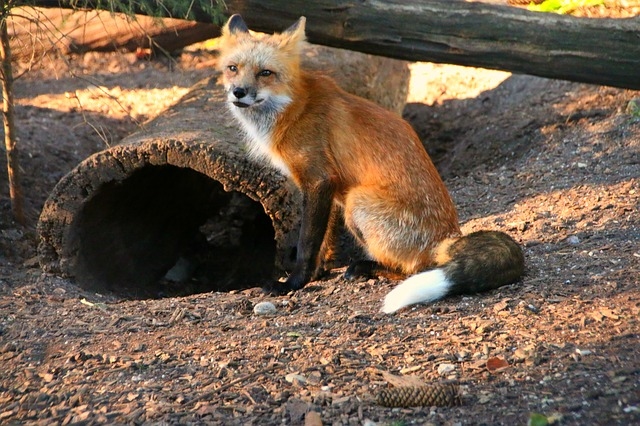
\includegraphics[height=3.0in]{images/fox_pixabay.jpg}
   \caption{Fox  on tunnel by pixabay}
 }

\maketitle

\begin{abstract}

A crucial element for the Red Team’s task is having stealth to perform the attack, success in the ability to expose an aggressive mindset and a true cracker’s point of view. If the red team win, they can help building a better defense for the Blue Team in the future. This content is meant for good purposes, don't worry.

At this paper, the content is about a different attack approach to get remote control of the machine and bypass the firewall.  We have a lot of weapons to work in that perspective, something like veil framework, msfvenom...  but sometimes following different  path,  will generally bring good result
\end{abstract}



\keywordlist

%% Required for all content. 


\section{The Basics of the attack }
The objective of the attack is to use Firefox to make all the communications between the client and the server by using hookings. This is not impossible, yet DLL injection sometimes can be boring to implement and even harder to make it portable. Did you know that x32 and x64 architecture need different approaches for development? (later I discovered that easyhook api can solve that). 
I was studying the firefox internals, reading something about the use of SQLite to work with cookies, that give to me a different focus.


Look that following:

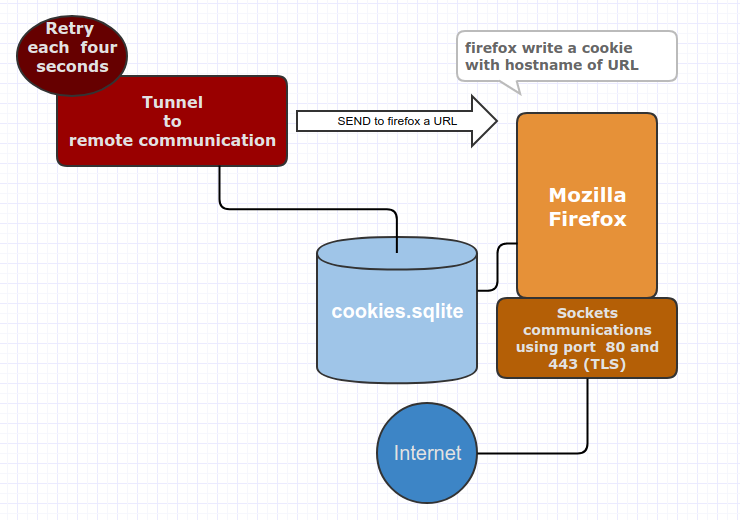
\includegraphics[height=2.5in]{images/tunnel4.png}



\section{Create the attack}

To create a program like firefox tunnel. These are the steps to get started:
\begin{itemize}
\item The program calls Firefox Browser in hidden mode, sends a URL that contains an evil server and finally that evil server sends a cookie with a command.
\item Tunnel gets the cookie of evil server (cookie.sqlite) and uses that to call a command shell.
\item The result of command shell is used to write an HTML with javascript to make auto submit with the content result.
\item The Programm opens HTML in hidden mode to send the result of CMD to the evil server.
\end{itemize}

Look that following:

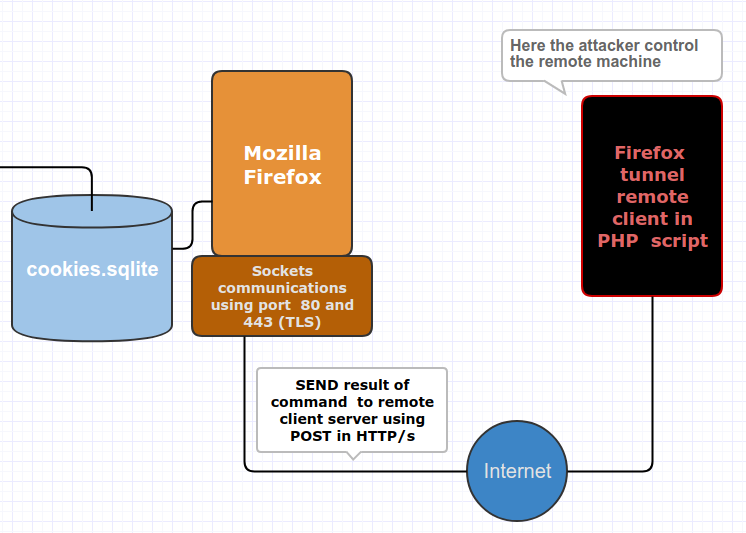
\includegraphics[height=2.5in]{images/tunnel8.png}



\section{The proof of concept}

In order to see this in action I have created a repository with everything you need and even a PoC. Please check the following link:
{\small\url{https://github.com/convisoappsec/firefox_tunnel}}

\section{Future insights}

\begin{itemize}
\item Insert persistence, using function RegOpenKeyEx() to  open path “Software/Microsoft/Windows/CurrentVersion/Run” and write with function RegSetValueEx() to launches a program automatically at system startup.
\item Use images in I/O using steganography.
\item Running process in  hidden mode.
\item Turn tunnel unkillable process.
\item Create DLL to inject in system process.
\item Function  to search different firefox binary path to execute.
\item Make portable to others browsers like chrome and IE.
\end{itemize}

\section{Possible mitigations}

\begin{itemize}
\item Global hooking, to get  OpenFile(), CreateFIle() functions and filter argv “cookie.sqlite” and block  when programm route is different of firefox.exe.
\item File watch api to monitor the database of cookies.
\item Programm to open database of cookies by periodicity and search evil domain or  hosts using query SELECT, that can use black list and uses DELETE query to remove the evil cookie.
\item Put firefox directory in different path.
\item Change firefox name of  binary file.
\item Programm to hooking SQLite and block non common querys.
\item Consult us for more ideas.
\end{itemize}


\section{Contact Information}

If you have questions or suggestions regarding this document, please
contact Antonio Costa at ``coolerlair@gmail.com'' or ``acosta@conviso.com.br''.

\section*{Acknowledgements}

Nash Leon for introducing me about headless trick.

Daniel Bermudez, Wagner Elias, Luan Souza aka p4ck4g3 for revision‏

\bibliographystyle{acmsiggraph}
\nocite{*}
\bibliography{template}
\end{document}
